
\section{Results}\label{results}
	\begin{figure*}[tb]
		\centering
		\includegraphics[width=0.5\linewidth,angle=-90]{figures/tonFigs/saturation-combined.eps}
		\caption{Simulation results under saturated traffic: a) Throughput under saturated conditions; b) Evolution of the fraction of collision slots in a scenario with 70 saturated stations; c) Average percentage of collision slots: fraction of time slots containing collisions; d) Average time between successful transmissions (sx tx), e) Throughput when increasing the clock drift probability}
		\label{fig:satResults}
	\end{figure*}
	
	%\begin{figure}[tb]
%	\centering
%		\includegraphics[width=0.7\linewidth,angle=-90]{figures/clockDrift/throughput_and_BOS_w_SD-TON.eps}
%		\caption{Throughput when increasing the clock drift probability}
%		\label{fig:clockDrift}
%	\end{figure}
	
	%\begin{figure*}[tb]
%	\centering
%		\subcaptionbox{Throughput under saturated conditions\label{fig:throughput-sat}}{\includegraphics[width=0.33\linewidth,angle=-90]{figures/saturated/throughput-saturated-w-BOS/throughput-saturated-w-BOS-TON.eps}}\hfill
%		\subcaptionbox{Average percentage of collision slots: the fraction of time slots containing collisions\label{fig:collisions-sat}}{\includegraphics[width=0.33\linewidth,angle=-90]{figures/saturated/collisions-saturated/collisions-saturated-TON.eps}}\\
%		\subcaptionbox{Evolution of the fraction of collision slots in a scenario with 70 saturated stations\label{fig:collisions-evolution}}{\includegraphics[width=0.33\linewidth,angle=-90]{figures/saturated/slots/Pc-evolution-TON.eps}}\hfill
%		\subcaptionbox{Average time between successful transmissions: averaging over all stations\label{fig:serviceTime-sat}}{\includegraphics[width=0.33\linewidth,angle=-90]{figures/saturated/timeBetweenSxTx-sat/timeBetweenSxTx-multiplot-sat-TON.eps}}\\
%		\caption{Saturated traffic results}
%		\label{fig:satTest}
%	\end{figure*}

	\subsection{Saturated nodes}\label{resultsSaturated}
	In CSMA/CA, a large number of saturated nodes will normally be related to a high collision probability. This effect is in part the result of resetting the backoff stage after a successful transmission and the generation of a new random backoff. However, this scenario provides an advantageous condition to CSMA/ECA$_{\text{Hys+FS}}$ nodes. In saturation, CSMA/ECA$_{\text{Hys+FS}}$ nodes build a collision-free schedule and stick to their deterministic backoff as long as they transmit successfully, effectively eliminating collisions.
	
	This section aims at overviewing the throughput of CSMA/CA and CSMA/ECA$_{\text{Hys+FS}}$ in saturation, as well as the collision probability, the average time between successful transmissions and the effect of clock drift over the throughput.
	\\
	\subsubsection{Throughput}
	CSMA/ECA$_{\text{Hys+FS}}$ nodes are able to build a collision-free schedule, use the channel more efficiently, and experience a throughput increase as seen in Figure~\ref{fig:satResults}a. Hysteresis allows the allocation of more contenders by increasing the length of the collision-free schedule, while Fair Share ensures an even distribution of the available throughput. This is reflected by the average backoff stage, which value increases with the number of contenders. In contrast, CSMA/CA throughput keeps decreasing due to an augmented number of collisions as the number of nodes increases (see Figure~\ref{fig:satResults}c). Further, Figure~\ref{fig:satResults}b shows the fraction of collision slots for CSMA/ECA$_{\text{Hys+FS}}$ and CSMA/CA as simulation time passes. In the figure, is appreciated how the fraction of collision slots keeps decreasing once CSMA/ECA$_{\text{Hys+FS}}$ reaches collision-free operation.


%	\begin{figure*}
%		\captionsetup{justification=raggedright}
%		\centering
%		\begin{minipage}[t]{0.45\textwidth}
%			\includegraphics[width=0.7\linewidth,angle=-90]{figures/saturated/throughput-saturated-w-BOS/throughput-saturated-w-BOS-TON.eps}
%			\caption{Throughput under saturated conditions}
%			\label{fig:throughput-sat}
%		\end{minipage}\hfill
%		\begin{minipage}[t]{0.45\textwidth}
%			\includegraphics[width=0.7\linewidth,angle=-90]{figures/saturated/collisions-saturated/collisions-saturated-TON.eps}
%			\caption{Average percentage of collision slots: the fraction of time slots containing collisions}
%			\label{fig:collisions-sat}
%		\end{minipage}\\
%		\begin{minipage}[t]{0.45\textwidth}
%			\includegraphics[width=0.7\linewidth,angle=-90]{figures/saturated/slots/Pc-evolution-TON.eps}
%			\caption{Evolution of the fraction of collision slots in a scenario with 70 saturated stations}
%			\label{fig:collisions-evolution}
%		\end{minipage}\hfill
%		\begin{minipage}[t]{0.45\textwidth}
%			\includegraphics[width=0.7\linewidth,angle=-90]{figures/saturated/timeBetweenSxTx-sat/timeBetweenSxTx-multiplot-sat-TON.eps}
%			\caption{Average time between successful transmissions: averaging over all stations}
%			\label{fig:serviceTime-sat}
%		\end{minipage}\hfill
%	\end{figure*}
	
%	\begin{figure}[tb]
%	\centering
%		\includegraphics[width=0.7\linewidth,angle=-90]{figures/saturated/throughput-saturated-w-BOS/throughput-saturated-w-BOS-TON.eps}
%		\caption{Throughput under saturated conditions}
%		\label{fig:throughput-sat}
%	\end{figure}
%	
%	\begin{figure}[tb]
%	\centering
%		\includegraphics[width=0.7\linewidth,angle=-90]{figures/saturated/collisions-saturated/collisions-saturated-TON.eps}
%		\caption{Average percentage of collision slots: the fraction of time slots containing collisions.}
%		\label{fig:collisions-sat}
%	\end{figure}
%	
%	\begin{figure}[tb]
%	\centering
%		\includegraphics[width=0.7\linewidth,angle=-90]{figures/saturated/slots/Pc-evolution-TON.eps}
%		\caption{Evolution of the fraction of collision slots in a scenario with 70 saturated stations.}
%		\label{fig:collisions-evolution}
%	\end{figure}
	
	\subsubsection{Effect of clock drift over the achieved throughput in saturation}\label{performanceClockDrift}
	Figure~\ref{fig:satResults}e shows the network aggregated throughput with 16 saturated stations and an increasing clock drift probability.
	
%	\begin{figure}[tb]
%	\centering
%		\includegraphics[width=0.7\linewidth,angle=-90]{figures/clockDrift/throughput_and_BOS_w_SD-TON.eps}
%		\caption{Throughput when increasing the clock drift probability}
%		\label{fig:clockDrift}
%	\end{figure}
	
	In Figure~\ref{fig:satResults}e, a station has a clock drift probability equal to $p_{cd}$. Each station has a probability of $p_{cd}/2$ of miscounting one slot more, and $p_{cd}/2$ of miscounting one slot less. Because CSMA/CA is based on a random backoff, miscounting slots has no significant effect on the throughput. For the CSMA/ECA curve, it is possible to appreciate a slight decrease of the throughput as $p_{cd}$ increases, caused by collisions due to the drift.
	
	The CSMA/ECA$_{\text{Hys+FS}}$ curve in Figure~\ref{fig:satResults}e shows instead an increase of the aggregated throughput as $p_{cd}$ grows. Collisions make CSMA/ECA$_{\text{Hys+FS}}$ contenders to increment their backoff stage and aggregate packets for transmissions according to Fair Share, effectively increasing the throughput. 
	
	As it also can be appreciated in the figure, the average backoff stage for CSMA/ECA$_{\text{Hys+FS}}$ contenders increases rapidly to its maximum value ($m=5$), reducing the effect of clock drift over CSMA/ECA$_{\text{Hys+FS}}$ nodes given that their transmissions would now be separated by more slots.\\
	
	\subsubsection{Time between successful transmissions}\label{timeBetweenSxTx}
	It is related to the elapsed time between the contention for transmission and the reception of an ACK.

%	\begin{figure}[tb]
%		\centering
%		\includegraphics[width=0.7\linewidth,angle=-90]{figures/saturated/timeBetweenSxTx-sat/timeBetweenSxTx-multiplot-sat-TON.eps}
%		\caption{Average time between successful transmissions: averaging over all stations}
%		\label{fig:serviceTime-sat}
%	\end{figure}
	
	In Figure~\ref{fig:satResults}d all tests with maximum aggregation, namely CSMA/CA$_{\text{MaxAg}}$ and CSMA/ECA$_{\text{Hys+MaxAg}}$, have an increased average time between successful transmissions. This is due to the multiple packets that are sent in each attempt. CSMA/CA$_{\text{MaxAg}}$, though, has an increased value due to collisions also taking longer channel time.
	
	Although CSMA/ECA$_{\text{Hys+FS}}$ has an increased average time between successful transmissions due to Fair Share, it has a lower metric when compared with the maximum aggregation curves in Figure~\ref{fig:satResults}d.


%	################################################################################################################


	\subsection{Non-saturated nodes}\label{resultsUnsaturated}
	
%	\begin{figure*}[tb]
%	\centering
%		\subcaptionbox{Throughput in non-saturation conditions\label{fig:throughputUnsat}}{\includegraphics[width=0.33\linewidth,angle=-90]{figures/unsaturated/throughput-unsaturated/throughput-unsaturated-w-BOS-TON.eps}}\hfill
%		\subcaptionbox{Average percentage of collision slots: the fraction of time slots containing collisions in non-saturated conditions\label{fig:collisions-unsat}}{	\includegraphics[width=0.33\linewidth,angle=-90]{figures/unsaturated/collision-unsaturated/collisions-unsaturated-TON.eps}}\\
%		\subcaptionbox{Average system delay: averaging over all stations\label{fig:serviceTime-unsat}}{\includegraphics[width=0.33\linewidth,angle=-90]{figures/unsaturated/queueingDelay/queueingDelay-TON.eps}}\hfill
%		\subcaptionbox{Average time between successful transmissions in non-saturated conditions: averaging over all stations\label{fig:timeBetweenSxTx-multiplot-unsat}}{\includegraphics[width=0.33\linewidth,angle=-90]{figures/unsaturated/timeBetweenSxTx-unsat/timeBetweenSxTx-multiplot-unsat-TON.eps}}\\
%		\caption{Non-saturated traffic results}
%		\label{fig:unsatTest}
%	\end{figure*}

	
	Emptying the MAC queue in CSMA/ECA$_{\text{Hys+FS}}$ means that nodes will reset their backoff stage to zero and use a random backoff when a new packet arrives at the queue, breaking any collision-free operation in CSMA/ECA$_{\text{Hys+FS}}$. The following show the impact over throughput, delay and time between successful transmissions when using CSMA/CA and CSMA/ECA$_{\text{Hys+FS}}$ in non-saturated conditions.\\
	
	\subsubsection{Throughput}
	
%   	\begin{figure}[tb]
%		\centering
%		\includegraphics[width=0.7\linewidth,angle=-90]{figures/unsaturated/throughput-unsaturated/throughput-unsaturated-w-BOS-TON.eps}
%		\caption{Throughput in non-saturation conditions}
%		\label{fig:throughputUnsat}
%	\end{figure}
	
	In Figure~\ref{fig:unsatResults}a, the aggregated throughput increases linearly for the \emph{CSMA/CA} curve until saturation is reached at around 22 nodes, where the throughput begins to degrade. The \emph{CSMA/ECA$_{\text{Hys+FS}}$} curve has a similar behavior, entering saturation at around 60 nodes. Further, at around 30 nodes we see an increase in the average backoff stage for CSMA/ECA$_{\text{Hys+FS}}$ contenders which suggests an increment in collisions. This effect is shown in Figure~\ref{fig:unsatResults}b and Figure~\ref{fig:unsatResults}d, where at around 35 nodes CSMA/ECA$_{\text{Hys+FS}}$ contenders start colliding and dropping packets. 
	
	\textcolor{black}{As indicated by Figure~\ref{fig:unsatResults}b, when $20<N\leq 35$ CSMA/ECA$_{\text{Hys+FS}}$ nodes suffer from an increasing number of  collisions. This is due to nodes emptying their MAC queue quicker due to Fair Share, as shown in Figure~\ref{fig:unsatResults}f and re-entering the contention with a random backoff every time a new packet arrives.} 
	
	\textcolor{black}{This increase in collisions may also cause the dropping of packets due to reaching the maximum retransmission limit. As CSMA/ECA$_{\text{Hys+FS}}$ drops more packets after reaching such limit (see line~\ref{discard} in Algorithm~\ref{alg:fullECA}), it shows a higher fraction of dropped packets in Figure~\ref{fig:unsatResults}d.}
	
	Beyond 35 contenders, the MAC queue of CSMA/ECA$_{\text{Hys+FS}}$ nodes starts to fill up, gradually allowing longer periods of collision-free operation due to CSMA/ECA$_{\text{Hys+FS}}$ nodes getting saturated. This allows CSMA/ECA$_{\text{Hys+FS}}$ to outperform CSMA/CA.\\
	
	\begin{figure*}[tb]
		\centering
		\includegraphics[width=0.5\linewidth,angle=-90]{figures/tonFigs/nonsaturation-combined.eps}
		\caption{Simulation results under non-saturated traffic: a) Throughput; b) Average percentage of collision slots: the fraction of time slots containing collisions; c) Average time between successful transmissions; d) Average fraction of dropped packets; e) Average system delay; f) Average number of packets in the MAC queue of a node}
		\label{fig:unsatResults}
	\end{figure*}
		
%   	\begin{figure}[tb]
%		\centering
%		\includegraphics[width=0.7\linewidth,angle=-90]{figures/unsaturated/collision-unsaturated/collisions-unsaturated-TON.eps}
%		\caption{Average percentage of collision slots: the fraction of time slots containing collisions in non-saturated conditions}
%		\label{fig:collisions-unsat}
%	\end{figure}	
	
	
	\subsubsection{Delay}
	
%	\begin{figure}[tb]
%		\centering
%		\includegraphics[width=0.7\linewidth,angle=-90]{figures/unsaturated/queueingDelay/queueingDelay-TON.eps}
%		\caption{Average system delay: averaging over all stations}
%		\label{fig:serviceTime-unsat}
%	\end{figure}
	
	This metric refers to the elapsed time between the injection of a packet into the station's MAC queue and the reception of an ACK for such packet. 
	
	In Figure~\ref{fig:unsatResults}e, a rapid increase in the delay for CSMA/CA nodes is appreciated at the saturation point (around 20 contenders), whereas CSMA/ECA$_{\text{Hys+FS}}$'s delay is still low. 
	
	\textcolor{black}{Further, with CSMA/ECA$_{\text{Hys+FS}}$ the percentage of blocked packets from the MAC queue is lower than CSMA/CA or CSMA/CA$_{\text{MaxAg}}$ (see Figure~\ref{fig:blocked-packets}). This is due to the construction of collision-free schedules which ensure that large A-MPDU transmissions do not suffer from collisions.}
	
	As CSMA/ECA$_{\text{Hys+FS}}$ nodes get saturated, the delay increases due to longer queueing and contention time (see the number of packets in the MAC queue for CSMA/ECA$_{\text{Hys+FS}}$ nodes in Figure~\ref{fig:unsatResults}f and how it is related to the increase in delay shown in Figure~\ref{fig:unsatResults}e).
	
%	\begin{figure}[tb]
%		\centering
%		\includegraphics[width=0.7\linewidth,angle=-90]{figures/unsaturated/timeBetweenSxTx-unsat/timeBetweenSxTx-multiplot-unsat-TON.eps}
%		\caption{Average time between successful transmissions in non-saturated conditions: averaging over all stations}
%		\label{fig:timeBetweenSxTx-multiplot-unsat}
%	\end{figure}	
	
	Figure~\ref{fig:unsatResults}c shows the average time between successful transmissions. It is possible to see from the figure that when CSMA/ECA$_{\text{Hys+FS}}$ approaches the saturation point the average time between successful transmissions increases, resembling Figure~\ref{fig:satResults}d. 
	
	\begin{figure}[tb]
		\centering
		\includegraphics[width=0.7\linewidth,angle=-90]{figures/unsaturated/blockingProb-unsat/blocking-unsaturated-TON.eps}
		\caption{Average fraction of blocked packets. When the MAC queue is full, packets comming from the uppers are discarded (or blocked) at the entrance of the buffer}
		\label{fig:blocked-packets}
	\end{figure}	
	
	%Moreover, this effect is related to an increase in collisions: colliding nodes should begin a new contention for a retransmission, which may result in a successful transmission or another collision, the latter further increasing the average time between successful transmissions.
	
%   	\begin{figure}[tb]
%		\centering
%		\includegraphics[width=0.7\linewidth,angle=-90]{figures/unsaturated/droppedPackets/droppedPacketsDueRET-TON.eps}
%		\caption{Percentage of droppped packets due to reaching the retransmission threshold. CSMA/ECA$_{\text{Hys+FS}}$ has an increased metric because the number of dropped packets is determined by Fair Share, i.e.: drops $2^{k}$ packets, where $k$ is the current backoff stage of the node}
%		\label{fig:droppedDueToRET}
%	\end{figure}
%	
%	 \begin{figure}[tb]
%		\centering				
%		\includegraphics[width=0.7\linewidth,angle=-90]{figures/unsaturated/queueSize/queueSize-multiplot-TON.eps}
%		\caption{Average number of packets in the MAC queue of a node}
%		\label{fig:MacQ}
%	\end{figure}
	
	%\\	
	\subsection{Coexistence with CSMA/CA}\label{coexistance-w-csmaca}
	
	\begin{figure*}[tb]
		\centering
		\includegraphics[width=0.5\linewidth,angle=-90]{figures/tonFigs/coexistence-combined.eps}
	\caption{Coexistence results: a) Network throughput when composed by various proportions of saturated CSMA/CA and CSMA/ECA$_{\text{Hys+FS}}$ nodes; b) Average percentage of collision slots for the tested saturated mixed network setups proportions; c) Network throughput when composed by various proportions of non-saturated CSMA/CA and CSMA/ECA$_{\text{Hys+FS}}$ nodes; d) Average percentage of collision slots for the tested mixed network setups proportions in non-saturated conditions; e) Average station throughput per MAC protocol in a saturated mixed network}
		\label{fig:coexResults}
	\end{figure*}
	
	
	CSMA/ECA is thought to be an evolution of CSMA/CA given its similarities and the ability to coexists with the latter. This section provides simulations results for a setup of different proportions of CSMA/CA nodes in a network where there are also CSMA/ECA$_{\text{Hys+FS}}$ contenders, that is: 1/4, 1/2 and 3/4 of the total nodes run CSMA/CA, while the rest uses CSMA/ECA$_{\text{Hys+FS}}$. This network configuration will be referred to as \emph{mixed network setup} from here on.	
	\subsubsection{Throughput}
	
	Figure~\ref{fig:coexResults}a shows the network throughput for different proportions of CSMA/CA nodes in a mixed network setup.
	
%	\begin{figure}[tb]
%		\centering
%		\includegraphics[width=0.7\linewidth,angle=-90]{figures/saturated/mixed/throughput-mixed/throughput-saturated-mixed-TON.eps}
%		\caption{Network throughput when composed by various proportions of CSMA/CA and CSMA/ECA$_{\text{Hys+FS}}$ nodes}
%		\label{fig:mixedThroughput-sat}
%	\end{figure}
%	
%	\begin{figure}[tb]
%		\centering
%		\includegraphics[width=0.7\linewidth,angle=-90]{figures/saturated/mixed/collisions-mixed/collisions-mixed-saturated-TON.eps}
%		\caption{Average percentage of collision slots for the tested mixed network setups proportions}
%		\label{fig:mixedCollisions-sat}
%	\end{figure}
%	
%	\begin{figure}[tb]
%		\centering
%		\includegraphics[width=0.7\linewidth,angle=-90]{figures/unsaturated/mixed/throughput-mixed/throughput-unsaturated-mixed-TON.eps}
%		\caption{Network throughput when composed by various proportions of non-saturated CSMA/CA and CSMA/ECA$_{\text{Hys+FS}}$ nodes}
%		\label{fig:mixedThroughput-unsat}
%	\end{figure}
%	
%	\begin{figure}[tb]
%		\centering
%		\includegraphics[width=0.7\linewidth,angle=-90]{figures/unsaturated/mixed/collisions-mixed/collisions-mixed-unsaturated-TON.eps}
%		\caption{Average percentage of collision slots for the tested mixed network setups proportions in non-saturated conditions}
%		\label{fig:mixCollisions-unsat}
%	\end{figure}
%	
%	\begin{figure}[tb]
%		\centering
%		\includegraphics[width=0.7\linewidth,angle=-90]{figures/saturated/mixed/throughput-per-protocol/throughput-per-protocol-TON.eps}
%		\caption{Average station throughput per MAC protocol in a saturated mixed network}
%		\label{fig:mixThroughput-sat-perProtocol-TON}
%	\end{figure}
	
	In the figure it is appreciated how the mixed network setups curves lay between the CSMA/CA and CSMA/ECA$_{\text{Hys+FS}}$ curves. As the proportion of CSMA/CA nodes decreases, the throughput increases as the result of a lower probability of collision, as can be seen in Figure~\ref{fig:coexResults}b. A similar behaviour is observed when testing the same proportion of nodes under non-saturated conditions. Figure~\ref{fig:coexResults}c and Figure~\ref{fig:coexResults}d show the average aggregated throughput and fraction of collisions slots in a non-saturated mixed network setup.
	
	As shown in Figure~\ref{fig:coexResults}a and Figure~\ref{fig:coexResults}c, at a lower proportion of CSMA/CA nodes ($1/4$) the average aggregated throughput is the greatest among the tested mixed network setups. This is because collisions trigger Hysteresis and Fair Share in CSMA/ECA$_{\text{Hys+FS}}$ nodes, lowering the number of times these nodes enter in a contention and reducing the overall collision probability when compared to an only CSMA/CA network (see Figure~\ref{fig:coexResults}b, Figure~\ref{fig:coexResults}d and Figure~\ref{fig:coexResults}e). As the proportion of CSMA/CA nodes increases, the network throughput approximates to CSMA/CA.
	
	\textcolor{black}{Figure~\ref{fig:coexResults}e shows the average throughput for CSMA/CA and CSMA/ECA$_{\text{Hys+FS}}$ stations in a saturated mixed setup (half the contenders using CSMA/CA). It is possible to see that for a low total number contenders ($N^{*}\leq 12$) CSMA/CA stations attain greater throughput than in a CSMA/CA-only network. Again, this is because in the mixed network setup the other $N^{*}/2$ contenders with CSMA/ECA$_{\text{Hys+FS}}$ use a deterministic backoff, leaving many empty slots between transmissions.} 
	
	\textcolor{black}{Still referring to Figure~\ref{fig:coexResults}e, for $N^{*}>12$ periods of collision-free operation and the aggregation performed with Fair Share allows CSMA/ECA$_{\text{Hys+FS}}$ to have larger channel time than CSMA/CA nodes, which throughput degrades even more than in CSMA/CA-only. These results suggests that a switch to CSMA/ECA$_{\text{Hys+FS}}$ can be beneficial for networks with high number of contenders.}
	
	
	%####################################################################################
	
	\textcolor{black}{\subsection{Channel errors and Schedule Reset}\label{resultsSchedRest}}
	
	\begin{figure*}[tb]
		\centering
		\includegraphics[width=0.65\linewidth,angle=-90]{figures/tonFigs/schedReset-combined.eps}
		\caption{Performance results with Schedule Reset. Curves called "aggr" reffer to values of $\gamma=1$, while "halv" refers to a schedule halving (see Section~\ref{aggr} and Algorithm~\ref{alg:schedRest}). \emph{dynStick} reffers to curvers where the node's stickiness is temporarily increased to two after a successful reduction of the schedule: a) Average throughput for a saturated network; b) Average throughput for a non-saturated network; c) Time between successful transmissions for a saturated network; d) Time between successful transmissions for a non-saturated network}
		\label{fig:SchedResetResults}
	\end{figure*}
	
	\textcolor{black}{Figure~\ref{fig:SchedResetResults}a shows the average aggregated throughput of a saturated network with a channel error probability, $p_e=0.1$ (see Section~\ref{channelErrorsDef}). We can see that the highest throughput, corresponding to CSMA/ECA$_{\text{Hys+FS}}$ is lower than the one observed in a perfect channel (Figure~\ref{fig:satResults}a). Furthermore, curves with Schedule Reset (SR) seem to have lower aggregated throughput. This is because the backoff stage, and therefore the level of aggregation done by Fair Share, is repeatedly reduced.}
	
	\textcolor{black}{Still assessing Figure~\ref{fig:SchedResetResults}a and focusing on the SR curves, we can see that both aggressive schedule halving with dynamic stickiness (\emph{SR aggr. halv. dynStick}) curves (with and without Fair Share) have higher aggregated throughput than the rest (for a description of aggressive schedule halving and dynamic stickiness, refer to Algorithm~\ref{alg:schedRest} and Section~\ref{aggr}). This Schedule Reset configuration reduces the time between successful transmissions (see Figure~\ref{fig:SchedResetResults}c) and mantains collision-free operation for longer periods of time thanks to the increase in the node's stickiness.}
	
	\textcolor{black}{Figure~\ref{fig:SchedResetResults}c shows the average time between successful transmissions for the same network setup. Even-though CSMA/ECA$_{\text{Hys+FS}}$ still has a higher metric than CSMA/CA due to the aggregation done by Fair Share, Schedule Reset is able of reducing this metric by almost $43\%$.}
	
	\textcolor{black}{Figure~\ref{fig:SchedResetResults}b and Figure~\ref{fig:SchedResetResults}d show the aggregated througput and time between successful transmissions, respectively for a non-saturated network with the same $p_e=0.1$. Since under non-saturated conditions CSMA/ECA$_{\text{Hys+FS}}$ nodes reset their schedule every time they empty their MAC queues, Schedule Reset's benefits are not relevant. Nevertheless, a reduction in the time between successful transmissions is observed for Schedule Reset curves in Figure~\ref{fig:SchedResetResults}d}.
	
	
	
	%\begin{figure}[tb]
%		\centering
%		\includegraphics[width=0.7\linewidth,angle=-90]{figures/tonFigs/throughput-sat-SR-TON.eps}
%		\caption{Average throughput for a saturated network with channel error ($p_e=0.1$). Curves called "aggr" reffer to values of $\gamma=1$, while "halv" refers to a schedule halving (see Section~\ref{aggr} and Algorithm~\ref{alg:schedRest}). \emph{dynStick} reffers to curvers where the node's stickiness is temporarily increased to two after a successful reduction of the schedule}
%		\label{fig:throughput-sat-SR}
%	\end{figure}
%	
%	\begin{figure}[tb]
%		\centering
%		\includegraphics[width=0.7\linewidth,angle=-90]{figures/tonFigs/timeBetSxTx-sat-SR-TON.eps}
%		\caption{Time between successful transmissions for a saturated network with channel error ($p_e=0.1$). Curves called "aggr" reffer to values of $\gamma=1$, while "halv" refers to a schedule halving (see Section~\ref{aggr} and Algorithm~\ref{alg:schedRest}). \emph{dynStick} reffers to curvers where the node's stickiness is temporarily increased to two after a successful reduction of the schedule}
%		\label{fig:timeBetSxTx-sat-SR}
%	\end{figure}
